% !TEX root = ../master_thesis.tex
\chapter{Compléments au chapitre~\ref{chap:T}}\label{annexe:T}

\section{Dérivation de la matrice $T$ à partir de la théorie de la perturbation à plusieurs corps}\label{annexe:défauts}

Cette annexe présente la dérivation complète de la matrice $T$ introduite à la section~\ref{sec:mbt_T} et suit la présentation du chapitre 11 de l'ouvrage de Bruus et Flensberg~\cite{bruusManyBodyQuantumTheory2004}. Nous partons de l'Hamiltonien de couplage entre les électrons et un défaut unique, puis appliquons la théorie de la perturbation à plusieurs corps pour obtenir la fonction de Green de Matsubara électronique dans le formalisme de la matrice $T$. Toutes les expressions données ici sont exprimées en unités atomiques d'Hartree, où
\begin{equation}
    \hbar = e = 4\pi\varepsilon_0 = m_e = k_B = 1.
    \label{eqn:ad_unités_hartree}
\end{equation}

Conformément à la section~\ref{sec:hamiltonien}, l'Hamiltonien électronique en présence d'un seul défaut se décompose en une partie libre et une partie de couplage. Comme nous travaillons à température finie, il est naturel de se placer dans l'ensemble grand canonique et de mesurer les énergies à partir du potentiel chimique $\mu$
\begin{equation}
    \hat{H}-\mu\hat{N} = \hat{H}_\text{e}+\hat{H}_\text{ed} = \sum_{n}\xi_{n}\hat{c}^\dag_{n}\hat{c}_{n}+\frac{1}{N_\text{uc}}\sum_{mn}M_{mn}\hat{c}^\dag_{m}\hat{c}_{n},\qquad \xi_n\equiv\varepsilon_n-\mu,
    \label{eqn:ad_hamiltonien}
\end{equation}
où $\varepsilon_{n}$ sont les énergies propres de Kohn-Sham du cristal parfait et où les éléments de matrice électron-défaut $M_{mn}$ contiennent les contributions locale et non locale obtenues au chapitre~\ref{chap:défauts}. Pour alléger la notation, nous avons omis les indices de vecteur d'onde : dans toute cette annexe, un indice latin $n$ désigne collectivement la bande \emph{et} le vecteur d'onde, $n\equiv(n,\kv)$. Cette convention est essentielle, car le défaut brise la symétrie de translation et $M_{mn}$ n'est pas diagonale en $\kv$ ; l'Hamiltonien non perturbé $\hat{H}_\text{e}$, lui, demeure diagonal dans cette base. Nous allons utiliser la théorie de la perturbation en mécanique quantique sur l'Hamiltonien de couplage pour résoudre ce problème.

Le lecteur peut s'interroger sur l'utilité d'employer la théorie de la perturbation pour ce problème, qui peut être résolu exactement. En effet, l'Hamiltonien de couplage est quadratique dans les opérateurs de création et d'annihilation électroniques, ce qui découle du fait qu'en présence d'un seul défaut, le problème se ramène essentiellement à un système à un corps. Cependant, un échantillon réaliste contient un grand nombre de défauts répartis aléatoirement, et les observables mesurées correspondent à une moyenne sur les configurations de désordre. Cette moyenne ne peut pas être effectuée exactement, et c'est précisément le langage diagrammatique qui permet de l'organiser en une série contrôlée par la concentration de défauts. Le formalisme développé ici pour un défaut unique en constitue la brique élémentaire. La quantité centrale dans la théorie de la perturbation à plusieurs corps est la fonction de Green de Matsubara du système perturbé
\begin{equation}
    \mathcal{G}_{mn}(\tau'-\tau) = -\frac{{}_{0}\langle\mathcal{T}\hat{c}_m(\tau')S
    (\beta, 0)\hat{c}^\dag_n(\tau)\rangle_0}{{}_{0}\langle S(\beta, 0) \rangle_0},\label{eqn:ad_G}
\end{equation}
où ${}_{0}\langle\dots\rangle_0$ est une moyenne thermique par rapport à l'Hamiltonien non perturbé $\hat{H}_\text{e}$, $\tau$ est un temps imaginaire, $\mathcal{T}$ est l'opérateur d'ordonnancement temporel (il ordonne les opérateurs dans le temps, avec le plus grand temps à gauche), $\beta=1/T$ est l'inverse de la température et où la matrice $S$ est définie formellement par
\begin{equation}
    S(\beta, 0) = \mathcal{T}\exp{-\int_0^\beta d\tau\, \hat{H}_\text{ed}(\tau)} = \sum_{p=0}^\infty \frac{(-1)^p}{p!}\int_0^\beta d\tau_1\dots\int_0^\beta d\tau_p\,\mathcal{T}\left[\hat{H}_\text{ed}(\tau_1)\dots\hat{H}_\text{ed}(\tau_p)\right],
\end{equation}
où les opérateurs $\hat{O}(\tau)$ sont écrits dans la représentation d'interaction. Pour évaluer la fonction de Green, nous développons la matrice $S$ en puissances de l'interaction $\hat{H}_\text{ed}$, utilisons le théorème de Wick~\cite{wickEvaluationCollisionMatrix1950} pour apparier les opérateurs électroniques, puis resommons la série ainsi engendrée à l'aide de diagrammes de Feynman.

Avant d'écrire la série perturbative pour la fonction de Green de Matsubara, il est utile de formuler quelques règles pour évaluer correctement les termes de cette série.
\begin{itemize}
    \item Premièrement, nous allons apparier les opérateurs électroniques deux à deux. Comme ces paires vont être moyennées thermiquement par rapport à $\hat{H}_\text{e}$, qui conserve le nombre d'électrons dans chaque état, les seules paires non nulles sont celles qui contiennent exactement un opérateur de création et un opérateur d'annihilation.
    \item De plus, pour une paire donnée ${}_{0}\langle \mathcal{T}\hat{c}_m(\tau')\hat{c}_n^\dag(\tau)\rangle_0$, l'effet de l'opérateur $\hat{c}^\dag_n(\tau)$ est de placer un électron dans l'état $n$. Comme $\hat{H}_\text{e}$ est diagonal dans cette base, il est impératif que l'opérateur d'annihilation enlève ce même électron pour que la moyenne soit non nulle, ce qui impose $m=n$. Ainsi,
    \[{}_{0}\langle \mathcal{T}\hat{c}_m(\tau')\hat{c}_n^\dag(\tau)\rangle_0=\delta_{mn}\, {}_{0}\langle \mathcal{T}\hat{c}_n(\tau')\hat{c}_n^\dag(\tau)\rangle_0.\]
    \item Les deux règles suivantes concernent l'ordonnancement temporel des opérateurs. Pour une paire évaluée à des temps différents, l'opérateur $\mathcal{T}$ fixe lui-même l'ordre et la paire redonne, par définition, la fonction de Green de Matsubara du système non perturbé
    \[{}_0\langle \mathcal{T}\hat{c}_m(\tau')\hat{c}^\dag_n(\tau)\rangle_0=-\delta_{mn} \mathcal{G}_n^{(0)}(\tau'-\tau),\qquad {}_0\langle \mathcal{T}\hat{c}^\dag_n(\tau)\hat{c}_m(\tau')\rangle_0=+\delta_{mn} \mathcal{G}_n^{(0)}(\tau'-\tau),\]
    où le signe de la deuxième égalité provient de la transposition de deux opérateurs fermioniques à l'intérieur de $\mathcal{T}$. Le signe moins de la première égalité, lui, vient de la définition~\eqref{eqn:ad_G} de la fonction de Green.
    \item Pour une paire évaluée à temps égal, l'ordre n'est plus fixé par les temps et la convention est que $\mathcal{T}$ place l'opérateur de création à gauche. La moyenne donne alors l'occupation de l'état, c'est-à-dire la distribution de Fermi-Dirac pour des fermions comme les électrons
    \[{}_0\langle\mathcal{T}\hat{c}^\dag_m(\tau)\hat{c}_n(\tau)\rangle_0=+\delta_{mn}f_n,\qquad {}_0\langle\mathcal{T}\hat{c}_m(\tau)\hat{c}^\dag_n(\tau)\rangle_0=-\delta_{mn}f_n,\qquad f_n=\frac{1}{e^{\beta\xi_n}+1}.\]
    \item Il est possible d'évaluer exactement la fonction de Green du système non perturbé. En temps imaginaire et dans l'espace des fréquences de Matsubara, elle vaut respectivement
    \begin{equation}
        \mathcal{G}^{(0)}_n(\tau) = -\left[\theta(\tau)(1-f_n)-\theta(-\tau)f_n\right]e^{-\xi_n\tau},\qquad \mathcal{G}^{(0)}_n(i\omega_j)=\frac{1}{i\omega_j-\xi_n},
        \label{eqn:G0}
    \end{equation}
    où $\theta$ est la fonction de Heaviside et où les fréquences de Matsubara fermioniques $\omega_j$ sont définies à l'équation~\eqref{eqn:G_tau}.
    \item Enfin, lorsque nous apparions des opérateurs fermioniques avec le théorème de Wick, il faut ajouter un signe moins par permutation nécessaire pour rendre adjacents les opérateurs d'une même paire. Cela devient rapidement lourd et il est très facile de faire des erreurs. Une façon plus visuelle est de relier les opérateurs appariés par une ligne et de compter le nombre de croisements : le signe de l'appariement est $(-1)^{\text{nombre de croisements}}$.
\end{itemize}

Voyons comment écrire la série pour la fonction de Green de Matsubara du système perturbé à l'aide des règles décrites ci-dessus. En principe, nous devons développer la matrice $S$ au numérateur et au dénominateur simultanément, ce qui devient intraitable très rapidement. Heureusement, en vertu du théorème des amas connexes (traduit de l'anglais \textit{linked-cluster theorem})~\cite{goldstoneDerivationBruecknerManyBody1957,blochDeterminationLetatFondamental1958}, les diagrammes engendrés par le développement du dénominateur annulent exactement les diagrammes déconnectés engendrés par celui du numérateur. Ainsi, il suffit de ne considérer que le développement du numérateur et de ne garder que les diagrammes connectés. Commençons par le numérateur de l'équation~\eqref{eqn:ad_G} et procédons ordre par ordre.

À l'ordre zéro, aucune puissance de l'interaction n'intervient et ce terme se réduit à
\begin{align}
    \mathcal{G}_{mn}^{(0)}(\tau'-\tau) &= -{}_0\langle\mathcal{T}\hat{c}_m(\tau')\hat{c}^\dag_n(\tau)\rangle_0,\notag\\
    &= -\delta_{mn}\,{}_0\langle\mathcal{T}\hat{c}_n(\tau')\hat{c}^\dag_n(\tau)\rangle_0,\notag\\
    &= \delta_{mn}\mathcal{G}^{(0)}_n(\tau'-\tau),
\end{align}
soit la fonction de Green de Matsubara du système non perturbé. Pour tracer le diagramme de Feynman qui représente ce terme, nous utilisons les symboles introduits pour la spectroscopie Raman à la figure~\ref{fig:règles_Raman} : une ligne pleine fléchée pour le propagateur électronique et un cercle barré d'une croix pour le vertex électron-défaut. La traduction d'un diagramme en expression mathématique obéit alors aux règles suivantes : à chaque ligne pleine associer un propagateur libre $\mathcal{G}^{(0)}_n$, à chaque vertex un élément de matrice $M_{mn}$, intégrer chaque temps interne sur $[0,\beta]$, sommer sur chaque indice interne et ajouter un facteur $(-1)$ par boucle fermée de fermions. Le diagramme d'ordre zéro est illustré à la figure~\ref{fig:dyson_ordre0}.
\begin{figure}[htbp]
    \centering
    % Diagramme de Feynman : terme d'ordre zéro de la série de Dyson
% pour la fonction de Green électronique en présence d'un défaut.
% Style identique aux diagrammes du chapitre Raman (tikz/e1.tex, tikz/pd.tex).
% Compatible pdflatex. Requiert : tikz, decorations.markings, arrows.meta, calc.
\begin{tikzpicture}[
    line/.style={thick},
    >=Stealth,
    fermion/.style={
      postaction={decorate},
      decoration={markings, mark=at position 0.55 with {\arrow{Stealth}}}
    },
]
  % --- propagateur libre ---
  \draw[line, fermion] (0,0) -- (4,0);
  \node[above=3pt] at (2,0) {$n$};

  % --- extrémités ---
  \node[below=4pt] at (0,0) {$\tau$};
  \node[below=4pt] at (4,0) {$\tau'$};
  \fill (0,0) circle (0.05);
  \fill (4,0) circle (0.05);
\end{tikzpicture}

    \caption[Diagramme de Feynman du terme d'ordre zéro de la série de Dyson.]{Diagramme de Feynman du terme d'ordre zéro de la série de Dyson. L'électron se propage librement dans la bande $n$, du temps $\tau$ au temps $\tau'$, sans interagir avec le défaut.}
    \label{fig:dyson_ordre0}
\end{figure}
Physiquement, ce diagramme représente un électron dans l'état $n$ au temps $\tau$ qui évolue jusqu'au temps $\tau'$ tout en restant dans le même état. C'est donc un électron qui se propage librement sans interagir avec le défaut. Ce diagramme est connecté.

Le terme d'ordre un s'écrit
\begin{align}
    \mathcal{G}_{mn}^{(1)}(\tau'-\tau) &= (-1)^2\int_0^\beta d\tau_1 \,{}_0\langle\mathcal{T}\hat{c}_m(\tau')\hat{H}_\text{ed}(\tau_1)\hat{c}^\dag_n(\tau)\rangle_0,\notag\\
    &= (-1)^2\sum_{m_1n_1}\int_0^\beta d\tau_1\,{}_0\langle\mathcal{T}\hat{c}_m(\tau')\hat{c}^\dag_{m_1}(\tau_1)\hat{c}_{n_1}(\tau_1)\hat{c}^\dag_n(\tau)\rangle_0\,M_{m_1n_1},
\end{align}
où le facteur $(-1)^2$ combine le signe moins de la définition~\eqref{eqn:ad_G} et celui du terme $p=1$ de la matrice $S$. D'après le théorème de Wick, seuls deux appariements sont non nuls. Ils sont représentés par
\begin{equation}
\begin{aligned}
\mathcal{G}_{mn}^{(1)}(\tau'-\tau)
= (-1)^2 \sum_{m_1n_1} \int_0^\beta &d\tau_1\,
\Big[
    {}_0\langle\mathcal{T}
      \wick{
        \c1 c_{m}(\tau')
        \c1 c_{m_1}^\dag(\tau_1)
        \c2 c_{n_1}(\tau_1)
        \c2 c_{n}^\dag(\tau)
      }\rangle_0
\\
&
    +
    {}_0\langle\mathcal{T}
    \wick{
        \c1 c_{m}(\tau')
        \c2 c_{m_1}^\dag(\tau_1)
        \c2 c_{n_1}(\tau_1)
        \c1 c_{n}^\dag(\tau)
    }\rangle_0
\Big]M_{m_1n_1}.
\end{aligned}
\end{equation}
Ici, les lignes de contraction ne se croisent dans aucun des deux cas : elles sont juxtaposées dans le premier terme et emboîtées dans le second. Les deux appariements portent donc un signe positif. Les appariements écrits explicitement sont
\begin{equation}
\begin{aligned}
\mathcal{G}_{mn}^{(1)}(\tau'-\tau)
= (-1)^2 \sum_{m_1n_1} \int_0^\beta &d\tau_1\,
\Big[
    {}_0\langle\mathcal{T}\hat{c}_{m}(\tau')\hat{c}_{m_1}^\dag(\tau_1)
      \rangle_0
      {}_0\langle\mathcal{T}\hat{c}_{n_1}(\tau_1)\hat{c}_{n}^\dag(\tau)
      \rangle_0
\\
&
    +
    {}_0\langle\mathcal{T}\hat{c}_{m}(\tau')\hat{c}_{n}^\dag(\tau)
      \rangle_0
      {}_0\langle\mathcal{T}\hat{c}_{m_1}^\dag(\tau_1)\hat{c}_{n_1}(\tau_1)
      \rangle_0
\Big]M_{m_1n_1}.
\end{aligned}
\end{equation}
Notons que, dans le second terme, la paire d'opérateurs à temps égal est écrite dans son ordre naturel, l'opérateur de création à gauche. Les moyennes thermiques des paires d'opérateurs sont ensuite évaluées selon les règles énoncées plus haut. Cela donne
\begin{equation}
\begin{aligned}
\mathcal{G}_{mn}^{(1)}(\tau'-\tau)
= \int_0^\beta &d\tau_1\,
\Big[
    \mathcal{G}^{(0)}_m(\tau'-\tau_1)M_{mn}\mathcal{G}^{(0)}_{n}(\tau_1-\tau)
\\
&
    -\delta_{mn}\sum_{n_1}\mathcal{G}_{n}^{(0)}(\tau'-\tau)f_{n_1} M_{n_1n_1}
\Big].
\end{aligned}
\end{equation}
Deux termes contribuent donc au premier ordre ; ils sont représentés par la somme des deux diagrammes de Feynman de la figure~\ref{fig:dyson_ordre1}.
\begin{figure}[htbp]
    \centering
    % Vertex électron-défaut : cercle blanc + croix (cf. tikz/règles_Raman.tex)
\providecommand{\vertexdefaut}[1]{%
  \draw[fill=white] (#1) circle (0.2);
  \draw[line width=1pt] ($(#1)+(-0.14,-0.14)$) -- ($(#1)+(0.14,0.14)$);
  \draw[line width=1pt] ($(#1)+(-0.14,0.14)$) -- ($(#1)+(0.14,-0.14)$);
}

\begin{tikzpicture}[
    line/.style={thick},
    >=Stealth,
    fermion/.style={
      postaction={decorate},
      decoration={markings, mark=at position 0.55 with {\arrow{Stealth}}}
    },
]

% ===================== (a) diagramme connecté =====================
\begin{scope}[shift={(0,0)}]
  \draw[line, fermion] (0,0)   -- (1.82,0);
  \draw[line, fermion] (2.18,0) -- (4,0);
  \node[above=3pt] at (0.9,0) {$n$};
  \node[above=3pt] at (3.1,0) {$m$};

  \vertexdefaut{2,0}
  \node[above=6pt] at (2,0) {$\tau_1$};
  \node[below=6pt] at (2,0) {$M_{mn}$};

  \node[below=4pt] at (0,0) {$\tau$};
  \node[below=4pt] at (4,0) {$\tau'$};
  \fill (0,0) circle (0.05);
  \fill (4,0) circle (0.05);

  \node[font=\small\bfseries] at (-0.6,1.6) {(a)};
\end{scope}

% ===================== (b) diagramme déconnecté =====================
\begin{scope}[shift={(7.2,0)}]
  \draw[line, fermion] (0,0) -- (4,0);
  \node[below=3pt] at (1.2,0) {$n$};

  % boucle fermée, centre (2,1.15), rayon 0.55
  \draw[line, fermion] (2,0.60) arc (-90:90:0.55);
  \draw[line, fermion] (2,1.70) arc (90:270:0.55);
  \node[left=3pt] at (1.45,1.15) {$n_1$};

  \vertexdefaut{2,1.70}
  \node[above=6pt] at (2,1.70) {$\tau_1$, $M_{n_1n_1}$};

  \node[below=4pt] at (0,0) {$\tau$};
  \node[below=4pt] at (4,0) {$\tau'$};
  \fill (0,0) circle (0.05);
  \fill (4,0) circle (0.05);

  \node[font=\small\bfseries] at (-0.6,1.6) {(b)};
\end{scope}

\end{tikzpicture}

    \caption[Diagrammes de Feynman des termes du premier ordre de la série de Dyson.]{Diagrammes de Feynman des termes du premier ordre de la série de Dyson. (a) Diagramme connecté : l'électron diffuse une fois sur le défaut au temps $\tau_1$, avec une amplitude $M_{mn}$. (b) Diagramme déconnecté : la boucle fermée au temps $\tau_1$ n'est reliée par aucun propagateur au reste du diagramme et est annulée par le dénominateur de l'équation~\eqref{eqn:ad_G}.}
    \label{fig:dyson_ordre1}
\end{figure}
Physiquement, le premier diagramme représente un électron dans l'état $n$ au temps $\tau$ qui se propage vers l'état $m$ au temps $\tau'$ en diffusant sur le défaut au temps $\tau_1$ avec une amplitude de probabilité $M_{mn}$. Le deuxième diagramme est déconnecté et nous pouvons l'ignorer.

Au deuxième ordre, le développement du numérateur s'écrit
\begin{align}
    \mathcal{G}^{(2)}_{mn}(\tau'-\tau) &= \frac{(-1)^3}{2!}\int_0^\beta d\tau_1\,\int_0^\beta d\tau_2\, {}_0\langle\mathcal{T}\hat{c}_m(\tau')\hat{H}_\text{ed}(\tau_1)\hat{H}_\text{ed}(\tau_2)\hat{c}^\dag_{n}(\tau)\rangle_0,\notag\\
    & = \frac{(-1)^3}{2!}\sum_{n_1m_1}\sum_{n_2m_2}\int_0^\beta d\tau_1\,\int_0^\beta d\tau_2\,\notag\\
    &\qquad\times {}_0\langle\mathcal{T}\hat{c}_m(\tau')\hat{c}_{m_1}^\dag(\tau_1)\hat{c}_{n_1}(\tau_1)\hat{c}_{m_2}^\dag(\tau_2)\hat{c}_{n_2}(\tau_2)\hat{c}_n^\dag(\tau)\rangle_0\,M_{m_1n_1}M_{m_2n_2}.
\end{align}
Nous avons maintenant six appariements non nuls. En général, pour $N$ paires d'opérateurs de création et d'annihilation fermioniques, leur nombre s'élève à $N!$. Ces appariements sont
\begin{align}
    \mathcal{G}_{mn}^{(2)}(\tau'-\tau) &= \frac{(-1)^3}{2!}\sum_{n_1m_1}\sum_{n_2m_2}\int_0^\beta d\tau_1\,\int_0^\beta d\tau_2\,\Big[\nonumber\\
    &\wick{{}_0\langle\mathcal{T} \c1 c_{m}(\tau') \c1 c_{m_1}^\dag(\tau_1) \c1 c_{n_1}(\tau_1) \c1 c_{m_2}^\dag(\tau_2) \c1 c_{n_2}(\tau_2) \c1 c_{n}^\dag(\tau)}\rangle_0\nonumber\\
    &+\wick{{}_0\langle\mathcal{T} \c1 c_{m}(\tau') \c1 c_{m_1}^\dag(\tau_1) \c1 c_{n_1}(\tau_1) \c2 c_{m_2}^\dag(\tau_2) \c2 c_{n_2}(\tau_2)\c1 c_{n}^\dag(\tau)}\rangle_0\nonumber\\
    &+\wick{{}_0\langle\mathcal{T} \c1 c_{m}(\tau') \c2 c_{m_1}^\dag(\tau_1) \c2 c_{n_1}(\tau_1) \c1 c_{m_2}^\dag(\tau_2) \c1 c_{n_2}(\tau_2) \c1 c_{n}^\dag(\tau)}\rangle_0\nonumber\\
    &+\wick{{}_0\langle\mathcal{T} \c1 c_{m}(\tau') \c2 c_{m_1}^\dag(\tau_1) \c3 c_{n_1}(\tau_1) \c1 c_{m_2}^\dag(\tau_2) \c2 c_{n_2}(\tau_2) \c3 c_{n}^\dag(\tau)}\rangle_0\nonumber\\
    &+\wick{{}_0\langle\mathcal{T} \c1 c_{m}(\tau')\c2 c_{m_1}^\dag(\tau_1)\c2 c_{n_1}(\tau_1)\c2 c_{m_2}^\dag(\tau_2)\c2 c_{n_2}(\tau_2) \c1 c_{n}^\dag(\tau)}\rangle_0\nonumber\\
    &+\wick{{}_0\langle\mathcal{T} \c1 c_{m}(\tau') \c2 c_{m_1}^\dag(\tau_1)\c3 c_{n_1}(\tau_1)\c3 c_{m_2}^\dag(\tau_2)\c2 c_{n_2}(\tau_2)\c1 c_{n}^\dag(\tau)}\rangle_0\Big]M_{m_1n_1}M_{m_2n_2}.
\end{align}
Seul le quatrième appariement présente des croisements, au nombre de trois : les trois lignes de contraction s'y coupent deux à deux. Tous les autres appariements sont formés de lignes juxtaposées ou emboîtées et ne présentent aucun croisement. Nous devons donc ajouter un signe moins uniquement au quatrième terme. En écrivant les paires d'opérateurs fermioniques explicitement, nous avons
\begin{align}
    \mathcal{G}^{(2)}_{mn}(\tau'-\tau) &= \frac{(-1)^3}{2!}\sum_{n_1m_1}\sum_{n_2m_2}\int_0^\beta d\tau_1\,\int_0^\beta d\tau_2\Big[\nonumber\\
    &{}_0\langle\mathcal{T}\hat{c}_{m}(\tau')\hat{c}_{m_1}^\dag(\tau_1)\rangle_0{}_0\langle\mathcal{T}\hat{c}_{n_1}(\tau_1)\hat{c}_{m_2}^\dag(\tau_2)\rangle_0{}_0\langle\mathcal{T}\hat{c}_{n_2}(\tau_2)\hat{c}_{n}^\dag(\tau)\rangle_0\nonumber\\
    &+{}_0\langle\mathcal{T}\hat{c}_{m}(\tau')\hat{c}_{m_1}^\dag(\tau_1)\rangle_0{}_0\langle\mathcal{T}\hat{c}_{n_1}(\tau_1)\hat{c}_{n}^\dag(\tau)\rangle_0{}_0\langle\mathcal{T}\hat{c}_{m_2}^\dag(\tau_2)\hat{c}_{n_2}(\tau_2)\rangle_0\nonumber\\
    &+{}_0\langle\mathcal{T}\hat{c}_{m}(\tau')\hat{c}_{m_2}^\dag(\tau_2)\rangle_0{}_0\langle\mathcal{T}\hat{c}_{m_1}^\dag(\tau_1)\hat{c}_{n_1}(\tau_1)\rangle_0{}_0\langle\mathcal{T}\hat{c}_{n_2}(\tau_2)\hat{c}_{n}^\dag(\tau)\rangle_0\nonumber\\
    &-{}_0\langle\mathcal{T}\hat{c}_{m}(\tau')\hat{c}_{m_2}^\dag(\tau_2)\rangle_0{}_0\langle\mathcal{T}\hat{c}_{m_1}^\dag(\tau_1)\hat{c}_{n_2}(\tau_2)\rangle_0{}_0\langle\mathcal{T}\hat{c}_{n_1}(\tau_1)\hat{c}_{n}^\dag(\tau)\rangle_0\nonumber\\
    &+{}_0\langle\mathcal{T}\hat{c}_{m}(\tau')\hat{c}_{n}^\dag(\tau)\rangle_0{}_0\langle\mathcal{T}\hat{c}_{m_1}^\dag(\tau_1)\hat{c}_{n_1}(\tau_1)\rangle_0{}_0\langle\mathcal{T}\hat{c}_{m_2}^\dag(\tau_2)\hat{c}_{n_2}(\tau_2)\rangle_0\nonumber\\
    &+{}_0\langle\mathcal{T}\hat{c}_{m}(\tau')\hat{c}_{n}^\dag(\tau)\rangle_0{}_0\langle\mathcal{T}\hat{c}_{m_1}^\dag(\tau_1)\hat{c}_{n_2}(\tau_2)\rangle_0{}_0\langle\mathcal{T}\hat{c}_{n_1}(\tau_1)\hat{c}_{m_2}^\dag(\tau_2)\rangle_0\Big]\nonumber\\
    &\times M_{m_1n_1}M_{m_2n_2},
\end{align}
où le signe moins du quatrième terme provient de ses trois croisements. Enfin, en évaluant les moyennes thermiques, nous obtenons
\begin{align}
    \mathcal{G}^{(2)}_{mn}(\tau'-\tau) &= \frac{1}{2}\int_0^\beta d\tau_1\,\int_0^\beta d\tau_2\Big[\nonumber\\
    &\sum_{n_1}\mathcal{G}^{(0)}_m(\tau'-\tau_1)M_{mn_1}\mathcal{G}^{(0)}_{n_1}(\tau_1-\tau_2)M_{n_1n}\mathcal{G}_n^{(0)}(\tau_2-\tau)\nonumber\\
    & -\sum_{n_2}\mathcal{G}^{(0)}_m(\tau'-\tau_1)M_{mn}\mathcal{G}^{(0)}_n(\tau_1-\tau)f_{n_2}M_{n_2n_2}\nonumber\\
    &-\sum_{n_1}\mathcal{G}^{(0)}_m(\tau'-\tau_2)M_{mn}\mathcal{G}^{(0)}_n(\tau_2-\tau)f_{n_1}M_{n_1n_1}\nonumber\\
    &+\sum_{n_2}\mathcal{G}^{(0)}_m(\tau'-\tau_2)M_{mn_2}\mathcal{G}_{n_2}^{(0)}(\tau_2-\tau_1)M_{n_2n}\mathcal{G}_n^{(0)}(\tau_1-\tau)\nonumber\\
    &+\delta_{mn}\sum_{n_1n_2}\mathcal{G}_n^{(0)}(\tau'-\tau)f_{n_1}M_{n_1n_1}f_{n_2}M_{n_2n_2}\nonumber\\
    &-\delta_{mn}\sum_{n_1n_2}\mathcal{G}^{(0)}_n(\tau'-\tau)M_{n_1n_2}\mathcal{G}_{n_1}^{(0)}(\tau_1-\tau_2)M_{n_2n_1}\mathcal{G}^{(0)}_{n_2}(\tau_2-\tau_1)
    \Big].
\end{align}
Ces six appariements se traduisent par les six diagrammes de Feynman de la figure~\ref{fig:dyson_ordre2}.
\begin{figure}[htbp]
    \centering
    % Vertex électron-défaut : cercle blanc + croix (cf. tikz/règles_Raman.tex)
\providecommand{\vertexdefaut}[1]{%
  \draw[fill=white] (#1) circle (0.2);
  \draw[line width=1pt] ($(#1)+(-0.14,-0.14)$) -- ($(#1)+(0.14,0.14)$);
  \draw[line width=1pt] ($(#1)+(-0.14,0.14)$) -- ($(#1)+(0.14,-0.14)$);
}

% Boucle fermée (tadpole) : #1 centre x, #2 centre y, #3 rayon, #4 indice de bande
\providecommand{\boucledefaut}[4]{%
  \draw[line, fermion] (#1,{#2-#3}) arc (-90:90:#3);
  \draw[line, fermion] (#1,{#2+#3}) arc (90:270:#3);
  \node[left=3pt] at ({#1-#3},#2) {$#4$};
  \vertexdefaut{#1,{#2+#3}}
}

% Extrémités du propagateur : #1 x gauche, #2 x droit
\providecommand{\bornes}[2]{%
  \node[below=4pt] at (#1,0) {$\tau$};
  \node[below=4pt] at (#2,0) {$\tau'$};
  \fill (#1,0) circle (0.05);
  \fill (#2,0) circle (0.05);
}

\begin{tikzpicture}[
    line/.style={thick},
    >=Stealth,
    fermion/.style={
      postaction={decorate},
      decoration={markings, mark=at position 0.55 with {\arrow{Stealth}}}
    },
]

\def\colL{0}
\def\colR{7.8}
\def\rowA{0}
\def\rowB{-3.9}
\def\rowC{-7.8}

% ===================== (a) double diffusion : tau_2 puis tau_1 =====================
\begin{scope}[shift={(\colL,\rowA)}]
  \draw[line, fermion] (0,0)   -- (1.4,0);
  \draw[line, fermion] (1.8,0) -- (3.0,0);
  \draw[line, fermion] (3.4,0) -- (4.8,0);
  \node[above=3pt] at (0.7,0) {$n$};
  \node[above=3pt] at (2.4,0) {$n_1$};
  \node[above=3pt] at (4.1,0) {$m$};

  \vertexdefaut{1.6,0}
  \node[above=9pt] at (1.6,0) {$\tau_2$};
  \node[below=6pt] at (1.6,0) {$M_{n_1n}$};

  \vertexdefaut{3.2,0}
  \node[above=9pt] at (3.2,0) {$\tau_1$};
  \node[below=6pt] at (3.2,0) {$M_{mn_1}$};

  \bornes{0}{4.8}
  \node[font=\small\bfseries] at (-0.7,2.2) {(a)};
\end{scope}

% ===================== (b) une diffusion (tau_1) + boucle (tau_2) =====================
\begin{scope}[shift={(\colR,\rowA)}]
  \draw[line, fermion] (0,0)   -- (2.2,0);
  \draw[line, fermion] (2.6,0) -- (4.8,0);
  \node[above=3pt] at (1.1,0) {$n$};
  \node[above=3pt] at (3.7,0) {$m$};

  \vertexdefaut{2.4,0}
  \node[below=6pt] at (2.4,0) {$\tau_1$, $M_{mn}$};

  \boucledefaut{2.4}{1.35}{0.55}{n_2}
  \node[above=6pt] at (2.4,1.90) {$\tau_2$, $M_{n_2n_2}$};

  \bornes{0}{4.8}
  \node[font=\small\bfseries] at (-0.7,2.2) {(b)};
\end{scope}

% ===================== (c) une diffusion (tau_2) + boucle (tau_1) =====================
\begin{scope}[shift={(\colL,\rowB)}]
  \draw[line, fermion] (0,0)   -- (2.2,0);
  \draw[line, fermion] (2.6,0) -- (4.8,0);
  \node[above=3pt] at (1.1,0) {$n$};
  \node[above=3pt] at (3.7,0) {$m$};

  \vertexdefaut{2.4,0}
  \node[below=6pt] at (2.4,0) {$\tau_2$, $M_{mn}$};

  \boucledefaut{2.4}{1.35}{0.55}{n_1}
  \node[above=6pt] at (2.4,1.90) {$\tau_1$, $M_{n_1n_1}$};

  \bornes{0}{4.8}
  \node[font=\small\bfseries] at (-0.7,2.2) {(c)};
\end{scope}

% ===================== (d) double diffusion : tau_1 puis tau_2 =====================
\begin{scope}[shift={(\colR,\rowB)}]
  \draw[line, fermion] (0,0)   -- (1.4,0);
  \draw[line, fermion] (1.8,0) -- (3.0,0);
  \draw[line, fermion] (3.4,0) -- (4.8,0);
  \node[above=3pt] at (0.7,0) {$n$};
  \node[above=3pt] at (2.4,0) {$n_2$};
  \node[above=3pt] at (4.1,0) {$m$};

  \vertexdefaut{1.6,0}
  \node[above=9pt] at (1.6,0) {$\tau_1$};
  \node[below=6pt] at (1.6,0) {$M_{n_2n}$};

  \vertexdefaut{3.2,0}
  \node[above=9pt] at (3.2,0) {$\tau_2$};
  \node[below=6pt] at (3.2,0) {$M_{mn_2}$};

  \bornes{0}{4.8}
  \node[font=\small\bfseries] at (-0.7,2.2) {(d)};
\end{scope}

% ===================== (e) propagation libre + deux boucles =====================
\begin{scope}[shift={(\colL,\rowC)}]
  \draw[line, fermion] (0,0) -- (4.8,0);
  \node[below=3pt] at (2.4,0) {$n$};

  \boucledefaut{1.3}{1.35}{0.55}{n_1}
  \node[above=6pt] at (1.3,1.90) {$\tau_1$, $M_{n_1n_1}$};

  \boucledefaut{3.5}{1.35}{0.55}{n_2}
  \node[above=6pt] at (3.5,1.90) {$\tau_2$, $M_{n_2n_2}$};

  \bornes{0}{4.8}
  \node[font=\small\bfseries] at (-0.7,2.2) {(e)};
\end{scope}

% ===================== (f) propagation libre + boucle à deux vertex =====================
\begin{scope}[shift={(\colR,\rowC)}]
  \draw[line, fermion] (0,0) -- (4.8,0);
  \node[below=3pt] at (2.4,0) {$n$};

  % boucle : centre (2.4,1.35), demi-axes 1.1 et 0.55
  \draw[line, fermion] (1.3,1.35) arc (180:0:1.1 and 0.55);
  \draw[line, fermion] (3.5,1.35) arc (0:-180:1.1 and 0.55);
  \node[above=2pt] at (2.4,1.90) {$n_2$};
  \node[below=2pt] at (2.4,0.80) {$n_1$};

  \vertexdefaut{1.3,1.35}
  \node[left=4pt] at (1.3,1.35) {$\tau_1$};
  \vertexdefaut{3.5,1.35}
  \node[right=4pt] at (3.5,1.35) {$\tau_2$};

  \node[font=\small\bfseries] at (-0.7,2.2) {(f)};
  \bornes{0}{4.8}
\end{scope}

\end{tikzpicture}

    \caption[Diagrammes de Feynman des termes du deuxième ordre de la série de Dyson.]{Diagrammes de Feynman des termes du deuxième ordre de la série de Dyson, dans l'ordre des six appariements de Wick. (a) et (d) sont les deux diagrammes connectés.}
    \label{fig:dyson_ordre2}
\end{figure}

De ces six diagrammes, seuls (a) et (d) sont connectés. Ils diffèrent par l'ordre temporel des deux diffusions sur le défaut. Cet ordre est toutefois arbitraire, puisque les temps $\tau_1$ et $\tau_2$ sont intégrés : les deux diagrammes sont donc égaux et leur somme annule le $2!$ au dénominateur du préfacteur des termes de deuxième ordre.

En théorie, nous devrions faire cet exercice pour tous les ordres. En pratique, les calculs deviennent lourds très rapidement, comme l'illustre déjà le deuxième ordre. Au lieu de nous perdre dans des calculs interminables, nous pouvons gagner du temps en reconnaissant une régularité : à l'ordre $N$, il y a $(N+1)!$ appariements et seuls $N!$ d'entre eux sont connectés. Qui plus est, ces $N!$ diagrammes connectés sont tous équivalents et annulent exactement le $N!$ au dénominateur du préfacteur de chaque ordre. Ainsi, en ne considérant que les diagrammes connectés, nous obtenons une série perturbative pour la fonction de Green de Matsubara du système perturbé, exprimée à l'aide de diagrammes de Feynman et illustrée à la figure~\ref{fig:G_Dyson} du chapitre~\ref{chap:T}.

Cette série de diagrammes est l'équation de Dyson pour la diffusion sur un seul défaut et peut être sommée exactement, ce qui n'est pas surprenant, car il s'agit bien d'un problème de diffusion à un corps. Généralement, dans le contexte de la diffusion sur des défauts, l'équation de Dyson est résolue en introduisant la matrice $T$, définie diagrammatiquement à la figure~\ref{fig:T_matrice} du chapitre~\ref{chap:T}.

La matrice $T$ pour un seul défaut joue essentiellement le même rôle que la \textit{self}-énergie électronique dans le contexte de l'interaction électron-électron ou électron-phonon : elle regroupe l'ensemble des insertions irréductibles qui peuvent être greffées sur le propagateur libre. En traduisant la première ligne de la figure~\ref{fig:T_matrice} à l'aide des règles de Feynman, nous obtenons la série
\begin{equation}
    T = M + M\,\mathcal{G}^{(0)}M + M\,\mathcal{G}^{(0)}M\,\mathcal{G}^{(0)}M+\dots,
    \label{eqn:T_serie}
\end{equation}
où les produits sont matriciels sur les indices $n$ et convolutifs sur le temps imaginaire. La deuxième ligne de la figure~\ref{fig:T_matrice} exprime la même série sous forme récursive
\begin{equation}
    T = M + M\,\mathcal{G}^{(0)}T.
    \label{eqn:T_recursive}
\end{equation}
Pour résoudre l'équation~\eqref{eqn:T_recursive}, il est commode de passer dans l'espace des fréquences de Matsubara~\cite{matsubaraNewApproachQuantumStatistical1955}, où les convolutions en temps imaginaire deviennent de simples produits. Comme le défaut est statique, $\bm M$ ne dépend pas de la fréquence et la matrice $T$ est alors diagonale en fréquence de Matsubara. Les fonctions de Green de Matsubara fermioniques étant antipériodiques sur l'intervalle $[0,\beta]$, c.-à-d. $\mathcal{G}(\tau+\beta)=-\mathcal{G}(\tau)$, elles se développent en série de Fourier sur les fréquences de Matsubara fermioniques $\omega_j$
\begin{equation}
    \mathcal{G}(\tau) = \frac{1}{\beta}\sum_{j}e^{-i\omega_j\tau}\mathcal{G}(i\omega_j),\qquad \omega_j\equiv \frac{(2j+1)\pi}{\beta},\quad j \in\mathbb{Z},\label{eqn:G_tau}
\end{equation}
où la fonction de Green de Matsubara fermionique dans l'espace des fréquences est définie par l'inverse de l'équation~\eqref{eqn:G_tau}
\begin{equation}
    \mathcal{G}(i\omega_j) = \int_0^\beta d\tau\, e^{i\omega_j\tau}\mathcal{G}(\tau).\label{eqn:G_w}
\end{equation}
En utilisant ce développement en série de Fourier, nous obtenons l'équation~\eqref{eqn:T_recursive} dans l'espace des fréquences de Matsubara
\begin{equation}
    T_{mn}(i\omega_j) = M_{mn}+\sum_{n_1}M_{mn_1}\mathcal{G}^{(0)}_{n_1}(i\omega_j)T_{n_1n}(i\omega_j),
    \label{eqn:T_indices}
\end{equation}
qui se résout formellement par une inversion de matrice
\begin{equation}
    T(i\omega_j) = \left[\mathbb{I}-M\,\mathcal{G}^{(0)}(i\omega_j)\right]^{-1}M.
    \label{eqn:T_fermee}
\end{equation}
La matrice $T$ est ensuite employée pour resommer l'équation de Dyson, comme l'illustre la figure~\ref{fig:dyson_T} du chapitre~\ref{chap:T}. Cette resommation à tous les ordres n'est pas un simple raffinement formel : elle est indispensable pour les défauts considérés dans ce mémoire. En effet, le potentiel induit par une lacune est si fort qu'il n'existe aucun petit paramètre justifiant la troncature de la série de Dyson à un ordre fini. Le formalisme de la matrice $T$, exact pour un défaut unique, demeure valide dans cette limite de couplage fort puisqu'il inclut les effets du défaut à tous les ordres.

Il est également possible d'exprimer analytiquement la fonction de Green de Matsubara du système perturbé en fonction de la matrice $T$, en traduisant la série de diagrammes de la figure~\ref{fig:dyson_T} à l'aide des règles de Feynman. Cela donne
\begin{equation}
    \mathcal{G}_{mn}(\tau'-\tau) = \delta_{mn}\mathcal{G}^{(0)}_n(\tau'-\tau) + \int_0^\beta d\tau_1\,\int_0^\beta d\tau_2\,\mathcal{G}^{(0)}_m(\tau'-\tau_2)T_{mn}(\tau_2-\tau_1)\mathcal{G}^{(0)}_n(\tau_1-\tau).
\end{equation}
Dans l'espace des fréquences de Matsubara, les convolutions deviennent des produits et la fonction de Green du système perturbé prend la forme algébrique
\begin{equation}
    \mathcal{G}_{mn}(i\omega_j) =\delta_{mn}\mathcal{G}_n^{(0)}(i\omega_j)+\mathcal{G}^{(0)}_m(i\omega_j)T_{mn}(i\omega_j)\mathcal{G}^{(0)}_n(i\omega_j),
    \label{eqn:G_T}
\end{equation}
ou encore, avec la forme explicite~\eqref{eqn:G0} des fonctions de Green du système non perturbé,
\begin{equation}
    \mathcal{G}_{mn}(i\omega_j) = \frac{\delta_{mn}}{i\omega_j-\xi_n}+\frac{T_{mn}(i\omega_j)}{(i\omega_j-\xi_m)(i\omega_j-\xi_n)}.
    \label{eqn:G_T_explicite}
\end{equation}

Enfin, les fonctions de Matsubara, définies aux fréquences imaginaires $i\omega_j$, ne sont pas directement les quantités mesurées : les fonctions de réponse physiques sont les fonctions dites \emph{retardées}, définies sur l'axe des fréquences réelles. Les deux sont toutefois reliées par une continuation analytique. La fonction de Matsubara $\mathcal{G}(i\omega_j)$ et la fonction retardée $\mathcal{G}^R(\varepsilon)$ sont les restrictions d'une même fonction $\mathcal{G}(z)$, analytique dans le demi-plan complexe supérieur, aux points $z=i\omega_j$ et $z=\varepsilon+i0^+$ respectivement. Sous la condition $\mathcal{G}(z)\to 0$ lorsque $|z|\to \infty$ (le théorème de Baym-Mermin~\cite{baymDeterminationThermodynamicGreens1961}), cette continuation analytique est unique. Comme nous disposons ici d'expressions fermées dans l'espace des fréquences de Matsubara, elle se réduit à la simple substitution
\begin{equation}
    i\omega_j\to \varepsilon+i\eta, \quad\eta \to 0^+,
\end{equation}
qui produit les quantités retardées $\mathcal{G}^R(\varepsilon)$ et $T^R(\varepsilon)$. Dans tout le mémoire, les quantités exprimées dans l'espace des fréquences réelles sont implicitement retardées ; l'exposant $R$ est donc désormais omis.

Il convient de souligner que cette continuation analytique est triviale ici, alors qu'elle constitue généralement un problème numérique délicat. En effet, lorsque la fonction de Green n'est connue que numériquement, sur un ensemble fini de fréquences de Matsubara, la continuation analytique vers l'axe réel est un problème mal posé. L'information spectrale est exponentiellement atténuée sur l'axe imaginaire, de sorte qu'un faible bruit sur les données engendre de grandes incertitudes sur $\mathcal{G}(\varepsilon)$. Des méthodes de régularisation telles que les approximants de Padé~\cite{vidbergSolvingEliashbergEquations1977} ou l'entropie maximale~\cite{jarrellBayesianInferenceAnalytic1996} sont alors nécessaires pour obtenir une fonction retardée physiquement admissible. Heureusement, rien de tel n'est requis ici, puisque nous disposons d'expressions analytiques fermées pour la fonction de Green~\eqref{eqn:G_T_explicite} et la matrice $T$~\eqref{eqn:T_fermee}.

\clearpage
\section{Convergence et vérifications de la matrice $T$}\label{sec:annexe_T_tests}

Cette section rassemble la dépendance en taille de super-cellule et les preuves de convergence du schéma de l'amas de la matrice $T$ du chapitre~\ref{chap:T} : le rayon de coupure, la grille de sortie, l'élargissement et la grille interne de la fonction de Green de l'amas. Le corps du chapitre (section~\ref{sec:T_results}) ne garde que les paramètres retenus et l'incertitude de taille.

\vspace*{\fill}
\begin{figure}[htbp]
    \centering
    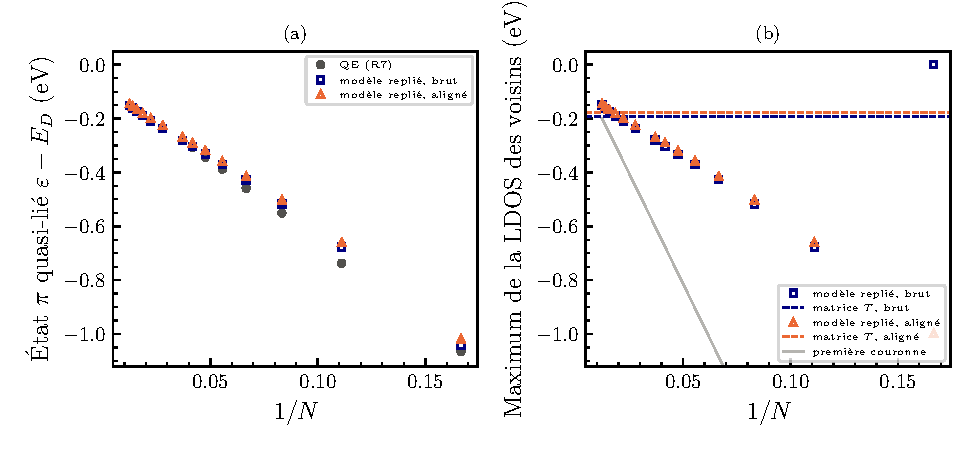
\includegraphics[width=\textwidth]{figures/fig_folded_vs_R7.pdf}
    \caption[Chaîne repliée dans la super-cellule et limite du défaut isolé.]{État $\pi$ quasi-lié de la lacune dans la super-cellule $N\times N$ au seul point $\Gamma$, en fonction de $1/N$. (a) Niveau obtenu par \texttt{QuantumESPRESSO} et par le modèle replié ($H(\Rv)$ et $\bm M$ interpolée, matrices brutes et alignées) pour $N=6$ à $27$. (b) Maximum de la densité d'états locale des voisins de la lacune dans le modèle replié, prolongé jusqu'à $N=81$ ; les lignes tiretées marquent la résonance de la matrice $T$ (grille interne $600^2$) et la ligne continue l'énergie de la première couronne d'états $\pi$ repliés sous $E_D$. La courbe alignée utilise la constante d'alignement à site unique $C_9=-24.65$~meV plutôt que celle de Kumagai-Oba ($-25.14$~meV), soit $0.5$~meV d'écart.}
    \label{fig:folded_vs_R7}
\end{figure}
\vspace*{\fill}
\clearpage
\vspace*{\fill}
\begin{figure}[htbp]
    \centering
    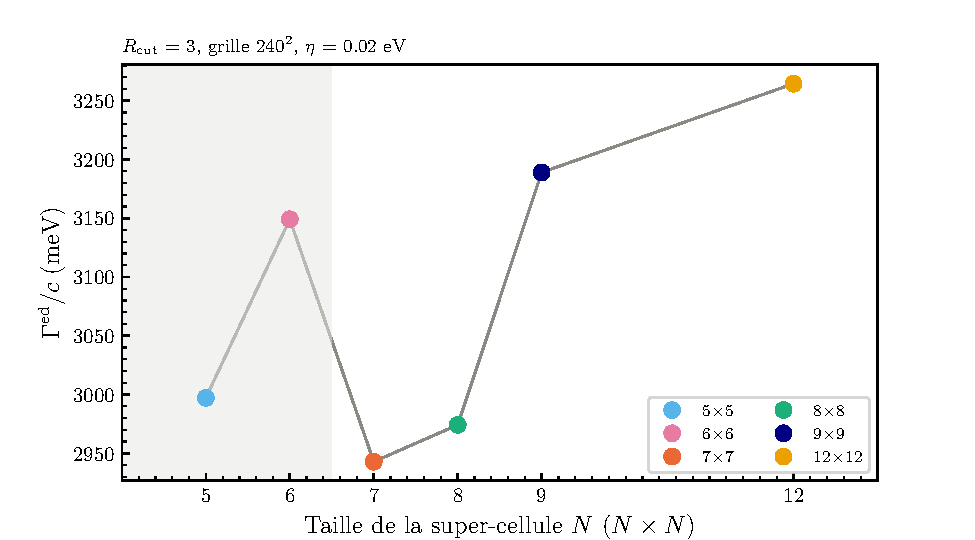
\includegraphics[width=\textwidth]{figures/fig_level2.pdf}
    \caption[Dépendance en taille de super-cellule du taux d'amortissement.]{Médiane de $\Gamma^\text{ed}/c$ sur $\pm3$~eV autour de $E_D$ en fonction de la taille $N$ de la super-cellule ayant servi à calculer $\bm M_\mathcal{C}$, aux paramètres de production ($R_\text{cut}=3$, grille de sortie $240\times240$, $\eta=20$~meV ; colonne $R_\text{cut}=3$ du tableau~\ref{tab:convergence_gamma}). La zone grisée marque les tailles $N<7$ exclues de la production. La dépendance n'est pas monotone : les deux familles de la section~\ref{sec:M_results} se séparent, $N=3m$ ($6$, $9$, $12$) au-dessus et les autres en dessous, et c'est au sein de la famille $3m$ que l'écart de $2.4~\%$ entre $9\times9$ et $12\times12$ retenu comme incertitude au chapitre~\ref{chap:T} se lit.}
    \label{fig:level2}
\end{figure}
\vspace*{\fill}
\clearpage
\vspace*{\fill}
\begin{table}[htbp]
    \centering
    \caption[Convergence du taux d'amortissement en fonction du rayon de
    coupure.]{Médiane de $\Gamma^\text{ed}/c$ (meV) sur $\pm3$~eV
    autour de $E_D$ en fonction du rayon de coupure $R_\text{cut}$, pour les
    six tailles de super-cellule (grille de sortie $240\times240$,
    $\eta = 20$~meV, grille interne $300\times300$). Nous distinguons les deux familles de super-cellules de la section~\ref{sec:M_results}.}
    \label{tab:convergence_gamma}
    % Généré par scripts/make_tables.py : ne pas éditer (python scripts/make_tables.py --only convergence_gamma).
% tab:convergence_gamma, §4.3.5 → annexe D. Valeurs et sources cellule par cellule : tables/SOURCES.md.
% Sources : M2_plateau/level1_summary.csv
\begin{tabular}{c c ccccc}
    \hline\hline
    $N$ & $N \bmod 3$ & $R_\text{cut}=0$ & 1 & 2 & 3 & 4 \\
    \hline
    6  & 0 & 3011 & 3243 & 3186 & 3149 & 3161 \\
    9  & 0 & 3014 & 3273 & 3222 & 3189 & 3200 \\
    12 & 0 & 3017 & 3299 & 3269 & 3265 & 3283 \\
    \hline
    5  & 2 & 2936 & 2966 & 2968 & 2997 & 2997 \\
    7  & 1 & 2929 & 2948 & 2946 & 2943 & 2953 \\
    8  & 2 & 2939 & 2991 & 2976 & 2974 & 2991 \\
    \hline\hline
\end{tabular}

\end{table}
\begin{figure}[htbp]
    \centering
    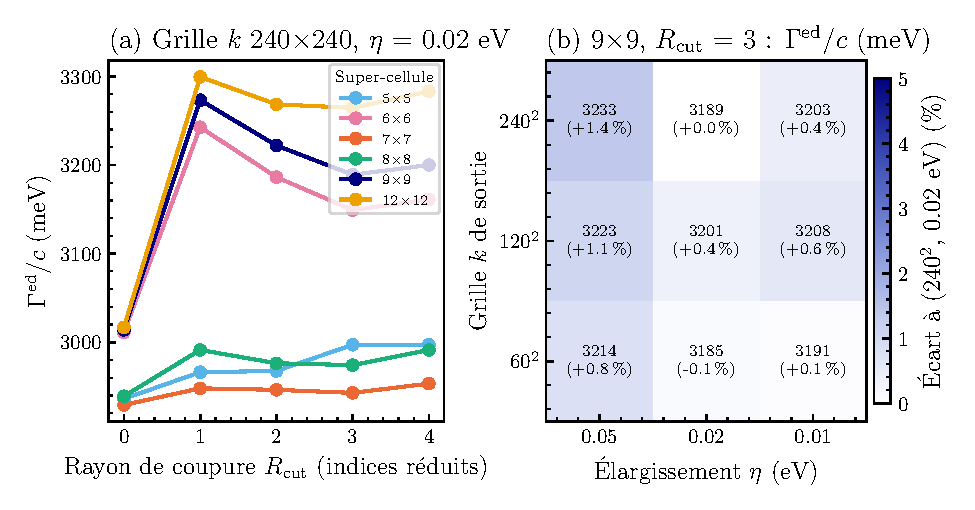
\includegraphics[width=\textwidth]{figures/fig_convergence.pdf}
    \caption[Convergence du taux d'amortissement par unité de
    concentration.]{Convergence de la médiane de $\Gamma^\text{ed}/c$
    sur $\pm3$~eV autour de $E_D$. (a) En fonction du rayon de coupure
    $R_\text{cut}$ du schéma de l'amas pour les six tailles de super-cellule,
    avec une grille de sortie $240\times240$ et un élargissement $\eta = 20$~meV. (b) En fonction de la grille de sortie et de $\eta$, pour la super-cellule de référence $9\times9$ à $R_\text{cut} = 3$. La couleur donne l'écart au point $(240^2, 20~\text{meV})$. La grille interne est de $300\times300$ ($N_{\tilde\kv}=300^2$) dans tous les cas.}
    \label{fig:convergence}
\end{figure}
\vspace*{\fill}

\clearpage
\vspace*{\fill}
\begin{table}[htbp]
    \centering
    \caption[Convergence du taux d'amortissement en grille interne.]{Convergence en grille interne $N_{\tilde\kv}$ de la fonction de Green de l'amas~\eqref{eqn:g_loc}, pour la super-cellule de référence $9\times9$ et les paramètres de production ($R_\text{cut}=3$, grille de sortie $240^2$, $\eta=20$~meV) : médiane de $\Gamma^\text{ed}/c$ sur la fenêtre $\pm3$~eV et sur la zone $|\varepsilon-E_D|\le0.3$~eV, taux d'amortissement des états situés au point de Dirac et position $E_\text{res}$ de la résonance, définie comme l'énergie de l'état de la grille de sortie où $\Gamma^\text{ed}/c$ est maximal.}
    \label{tab:grille_interne}
    \begin{tabular}{c c c c c}
    \hline\hline
    & \multicolumn{2}{c}{Médiane de $\Gamma^\text{ed}/c$ (meV)} & $\Gamma^\text{ed}/c\,(E_D)$ & $E_\text{res}-E_D$ \\
    \cline{2-3}
    $N_{\tilde\kv}$ & $\pm3$~eV & $\pm0.3$~eV & (meV) & (eV) \\
    \hline
    $150^2$ & 3210 & 4289 & 5662 & $-0.238$ \\
    $300^2$ & 3189 & 3045 & 4287 & $-0.175$ \\
    $450^2$ & 3196 & 3080 & 4120 & $-0.175$ \\
    $600^2$ & 3192 & 3039 & 4090 & $-0.175$ \\
    \hline\hline
\end{tabular}

\end{table}
\begin{figure}[htbp]
    \centering
    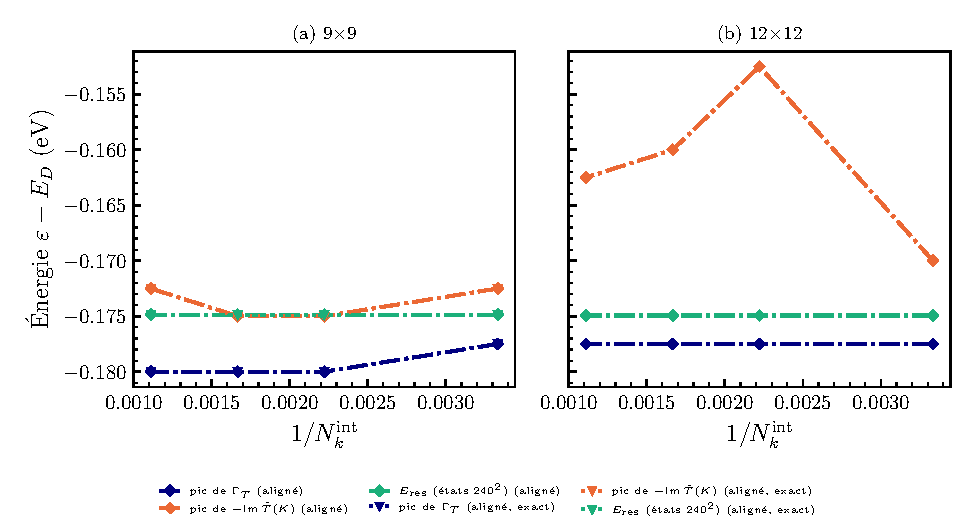
\includegraphics[width=\textwidth]{figures/fig_resonance_vs_nkint_plateau.pdf}
    \caption[Position de la résonance en fonction de la grille interne.]{Position de la résonance de la lacune en fonction de l'inverse de la grille interne $N_k^\text{int}=N_{\tilde\kv}$, pour les super-cellules (a) $9\times9$ et (b) $12\times12$ et les matrices alignées, avec les paramètres de production : pic de la courbe $\Gamma_T(\varepsilon)$ obtenue par la moyenne lorentzienne~\eqref{eqn:moyenne_lorentzienne}, pic de $-\mathrm{Im}\,\bar T(K;\varepsilon)$ et $E_\text{res}$ (état de la grille de sortie $240^2$ où $\Gamma^\text{ed}/c$ est maximal). Pour $9\times9$, l'alignement appliqué aux blocs diagonaux de la base de Wannier (section~\ref{sec:M_détails}) et l'alignement exact du potentiel se superposent.}
    \label{fig:resonance_vs_nkint_plateau}
\end{figure}
\vspace*{\fill}

\clearpage
\vspace*{\fill}
\begin{table}[htbp]
    \centering
    \small
    \setlength{\tabcolsep}{4pt}
    \caption[Vérifications du schéma de l'amas.]{Vérifications de la chaîne
    de calcul de la matrice $T$ et du taux d'amortissement par le schéma de l'amas : les tests et la quantité qu'ils contrôlent, la valeur obtenue et le seuil d'acceptation. Le test de
    référence compare le schéma de l'amas à l'inversion dense de
    l'équation~\eqref{eqn:T_chap} dans le sous-espace des cinq fonctions
    de Wannier, pour la super-cellule $5\times5$. Le test de $\mathcal{G}^{(0)}_\mathcal{C}$ par lots compare la fonction de Green de l'amas~\eqref{eqn:g_loc} construite par lots d'énergies à son évaluation directe ; la positivité est vérifiée sur les états de la fenêtre $\pm3$~eV de la super-cellule de référence $9\times9$.}
    \label{tab:tests_T}
    % Généré par scripts/make_tables.py : ne pas éditer (python scripts/make_tables.py --only tests_T).
% tab:tests_T, §4.2.5 → annexe D. Valeurs et sources cellule par cellule : tables/SOURCES.md.
% Sources : M2_plateau/M_tests_summary.csv ; M2_plateau/nkint_check_9x9.csv ; M2_plateau/resonance_9x9.npz ; ch4/NOTES_TGAMMA.md
\begin{tabular}{l l l l}
    \hline\hline
    Test & Quantité & Valeur & Seuil \\
    \hline
    Référence, $5\times5$           & $\max|\Gamma_\text{loc}-\Gamma_\text{dense}|/\max\Gamma$ & $1.8\times10^{-13}$ & $10^{-8}$ \\
    Grille interne, $300^2\to600^2$ & écart rel. sur la médiane                                & $9.1\times10^{-4}$  & --- \\
    Positivité                      & $\min_{n\kv}\Gamma_{n\kv}N_\text{cells}$                 & $1.96$~eV           & $-10^{-8}$~eV \\
    \hline\hline
\end{tabular}

\end{table}
\begin{figure}[htbp]
    \centering
    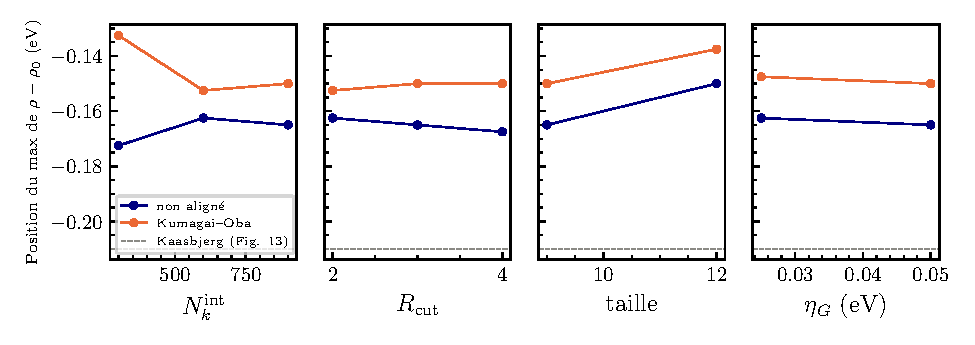
\includegraphics[width=\textwidth]{figures/fig_kaasbjerg_sensibilites.pdf}
    \caption[Sensibilité de la position du maximum de $\bar\rho-\rho_0$.]{Position du maximum de $\bar\rho-\rho_0$ de la densité d'états moyennée sur le désordre, à $c=1~\%$, en fonction de la grille interne, du rayon de coupure $R_\text{cut}$, de la taille de la super-cellule et de l'élargissement $\eta_G$, pour les matrices brutes et alignées. Les tirets marquent la valeur déduite de la figure 13 de Kaasbjerg~\cite{kaasbjergAtomisticMatrixTheory2020}, $-0.21$~eV.}
    \label{fig:kaasbjerg_sensibilites}
\end{figure}
\vspace*{\fill}
\clearpage
\vspace*{\fill}
\begin{figure}[htbp]
    \centering
    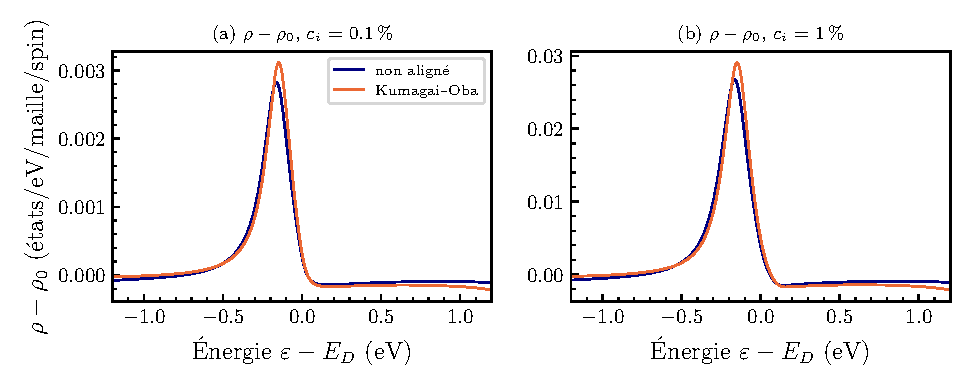
\includegraphics[width=\textwidth]{figures/fig_kaasbjerg_dos_c.pdf}
    \caption[Variation de la densité d'états moyennée sur le désordre.]{Variation $\bar\rho-\rho_0$ de la densité d'états moyennée sur le désordre, grille $600^2$, $\eta_G=50$~meV, pour (a) $c=0.1~\%$ et (b) $c=1~\%$, matrices brutes et alignées de la super-cellule $9\times9$ ; c'est la quantité dont le tableau~\ref{tab:kaasbjerg} rapporte la position, la hauteur et la largeur du maximum.}
    \label{fig:kaasbjerg_dos_c}
\end{figure}
\vspace*{\fill}

\clearpage
\section{Paramètres}\label{sec:annexe_param_T}

\vspace*{\fill}
\begin{table}[htbp]
    \centering
    \caption[Paramètres de la matrice $T$ et du taux d'amortissement $\Gamma^\text{ed}$.]{Paramètres du schéma de l'amas pour la matrice $T$ et le taux d'amortissement $\Gamma^\text{ed}$ (chapitre~\ref{chap:T}).}
    \label{tab:param_T}
    \small
    \setlength{\tabcolsep}{4pt}
    \begin{tabular}{p{0.27\textwidth} p{0.46\textwidth} p{0.14\textwidth}}
        \hline\hline
        Paramètre & Valeur & Section \\
        \hline
        Rayon de coupure $R_\text{cut}$ & $3$ & \ref{sec:T_détails} \\
        Nombre de cellules $N_L$ & $29$ (suite $1, 5, 13, 29, 49$ pour $R_\text{cut} = 0, \dots, 4$) & \ref{sec:T_détails} \\
        Nombre de fonctions de Wannier $N_W$ & $5$, soit une dimension $N_LN_W = 145$ & \ref{sec:T_détails} \\
        Grille interne $N_{\tilde\kv}$ & $300\times 300$ & \ref{sec:T_détails} \\
        Élargissement $\eta$ & $0.02$~eV & \ref{sec:T_détails} \\
        Grille de sortie $N_{\kv_f}$ & $240\times 240$, centrée sur $\Gamma$ & \ref{sec:T_détails} \\
        Fenêtre d'énergie & $\pm 3$~eV autour de $E_D$, soit $41\,266$ états & \ref{sec:T_détails} \\
        Pas de la grille d'énergie & $\eta/n_e$ avec $n_e = 8$, soit $2.5$~meV & \ref{sec:T_détails} \\
        Point de Dirac $E_D$ & $-4.239$~eV & \ref{sec:T_détails} \\
        Super-cellule de référence & $9\times 9$, grille élargie $27\times 27$ & \ref{sec:T_results} \\
        Moyenne lorentzienne & $\eta = 0.02$~eV & \ref{sec:T_results} \\
        Concentration de référence $c$ & $1~\%$ & \ref{sec:T_results} \\
        Comparaison avec Kaasbjerg & grille interne $900^2$ ; $\eta_G = 50$~meV ($\bar\rho - \rho_0$, grille $600^2$) et $25$~meV ($\bar A_\kv$) ; $\rho_0$ sur $1200^2$ avec $15$~meV ; $c = 0.1$ et $1~\%$ & \ref{sec:T_results} \\
        \hline\hline
    \end{tabular}
\end{table}
\vspace*{\fill}
